\subsection{Time projection chamber}
\writer{Paul Colas, Akira Sugiyama}{3}

The ILD TPC R\&D is being conducted mainly within the LCTPC Collaboration \cite{ild:bib:TPC_lctpc}. 

The workhorse for validation of detector prototypes and operational conditions is the TPC test set-up installed permanently in the DESY test beam\cite{ild:bib:TPC_desytb} (Figure~\ref{fig:det:TPC_test_setup}). The TPC stands within a magnet providing a magnetic field of 1 Tesla, and the beam line is equipped with precise incident and outgoing particle beam telescopes allowing to quantify the TPC reconstruction precision as function of the particle parameters. The beam test set up is currently being upgraded with the high precision LYCORIS silicon telescope~\cite{ild:bib:TPC_lycoris}, and a new TPC field cage with reduced field distortion is being assembled.

\begin{figure}[t!]
\centering
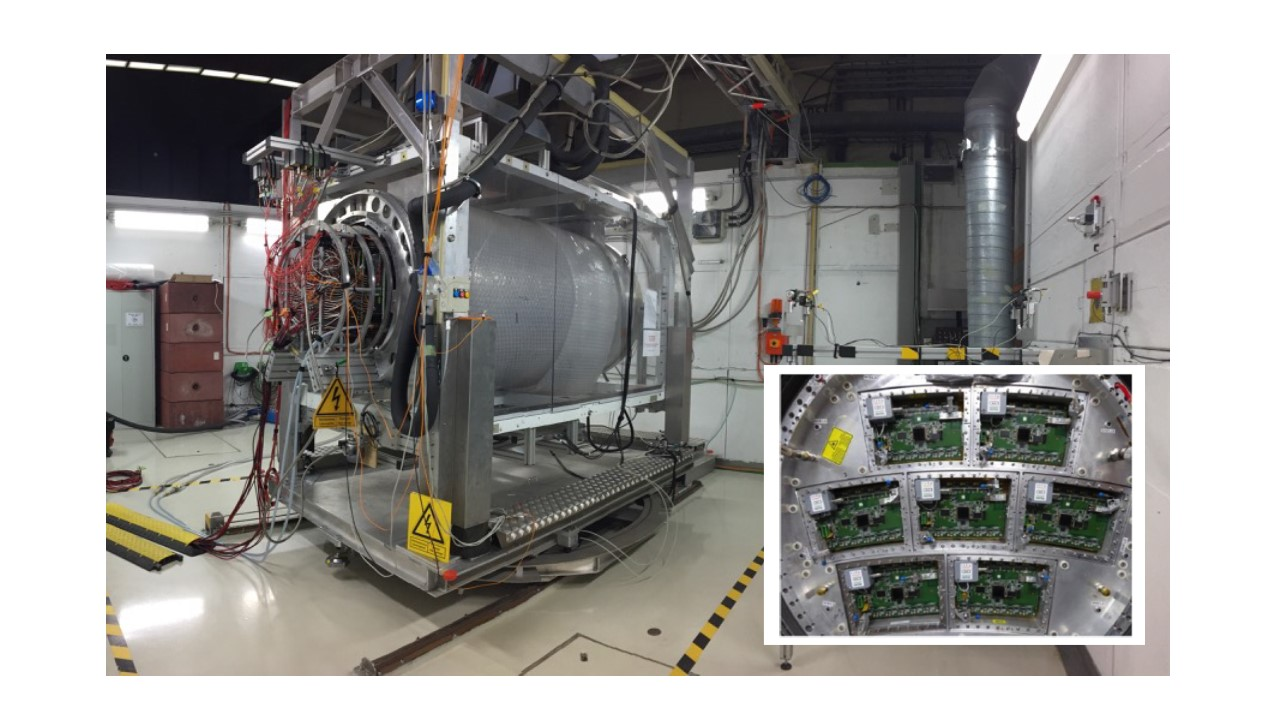
\includegraphics[width=1.0\hsize]{Detector/fig/TPC_test_setup.jpg}
\caption{The TPC test setup at DESY. The insert shows the geometrical structure of the TPC end cap which can host prototypes of detection planes.}
\label{fig:det:TPC_test_setup}
\end{figure}

Significant progress has been seen in the manufacturing process of detection modules for each of the readout options. A new micromegas layout with resistive anodes has been shown to exhibit reduced boundary distortions\cite{ild:bib:TPC_distortions}. The flatness of the GEM modules has been improved significantly, increasing the gain uniformity by a factor 2 [ref]. Operational GridPix "QUAD" modules have been built based on the TimePix3 pixel chip\cite{ild:bib:TPC_quad}. Recent prototypes of the three types of detection modules are shown in Figure~\ref{fig:det:TPC_prototypes}.  

\begin{figure}[t!]
\centering
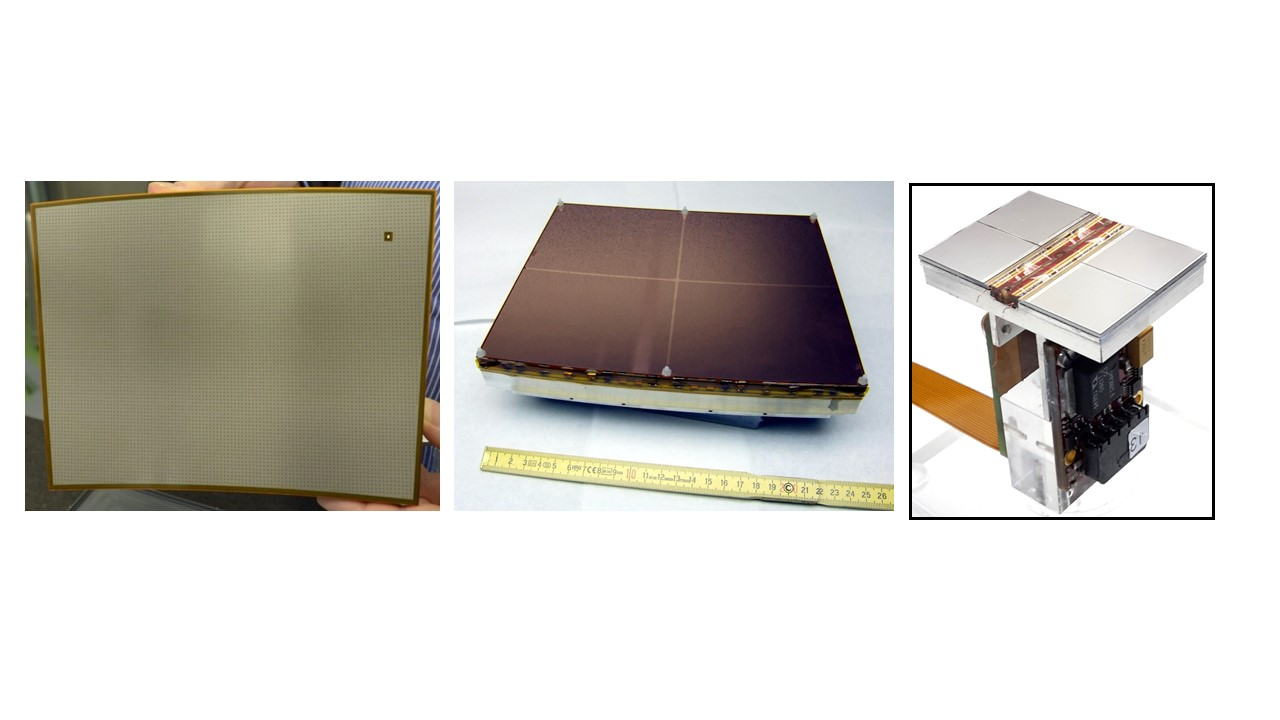
\includegraphics[width=1.0\hsize]{Detector/fig/TPC_prototypes.jpg}
\caption{TPC prototype detection modules for the three baseline technologies under consideration: micromegas module (left), GEM module (middle) and GridPix QUAD module (right).}
\label{fig:det:TPC_prototypes}
\end{figure}

The performance of the three technologies has been measured in beam tests. Figure~\ref{fig:det:TPC_performances} shows the measured point resolution in 1 T magnetic field for drift distances from 0 to 0.6 m. This can be safely extrapolated to $\sim~100$ $\mu$m in a field of 3.5~T at a drift length of 2.3~m. The dE/dx resolution by the truncated mean method has been measured to be respectively $4.6\%, 4.5\%$ and $4.2\%$ for Micromegas, GEM and GridPix technologies. It improves to $3.8\%$ for GridPix using a cluster counting method. The conclusion is that the target goals of a spatial resolution of 100 microns and of a dE/dx resolution better than 5\% have been reached in all cases.   

\textit{Q: add performance plot of 2 track separation?}

\begin{figure}[t!]
\centering
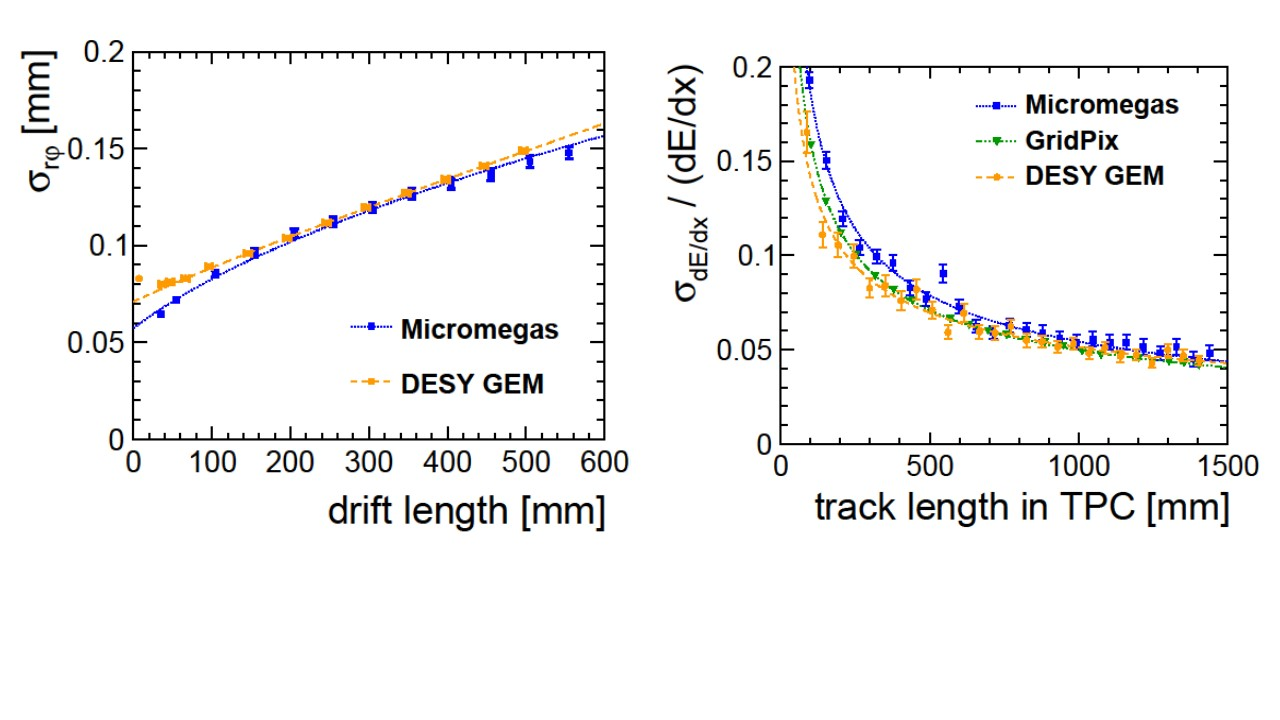
\includegraphics[width=1.0\hsize]{Detector/fig/TPC_performances.jpg}
\caption{Resolution on the track position in r$\phi$ (left) as function of the drift length and resolution on the ionisation loss dE/dx (right) as function of the track length, for the three readout options under consideration.}
\label{fig:det:TPC_performances}
\end{figure}

\vspace{1cm}
Two critical aspects of a TPC operation consist in the cooling of the readout endcaps, which must be realized with minimal dead material, and the mitigation of the drift field distortions which may develop from the accumulation of ions in the drift volume. For the first point a double phase $CO_2$ cooling system with thin low-material fluid pipes has been developed and shown to perform adequately (Figure~\ref{fig:det:TPC_operation} left). For the second point an ion gating scheme based on GEM foils has been implemented and beam tested. Results show that a good transparency for drift electron signals can be maintained while preventing the accumulation of ions in the drift volume (Figure~\ref{fig:det:TPC_operation} right).   

\begin{figure}[t!]
\centering
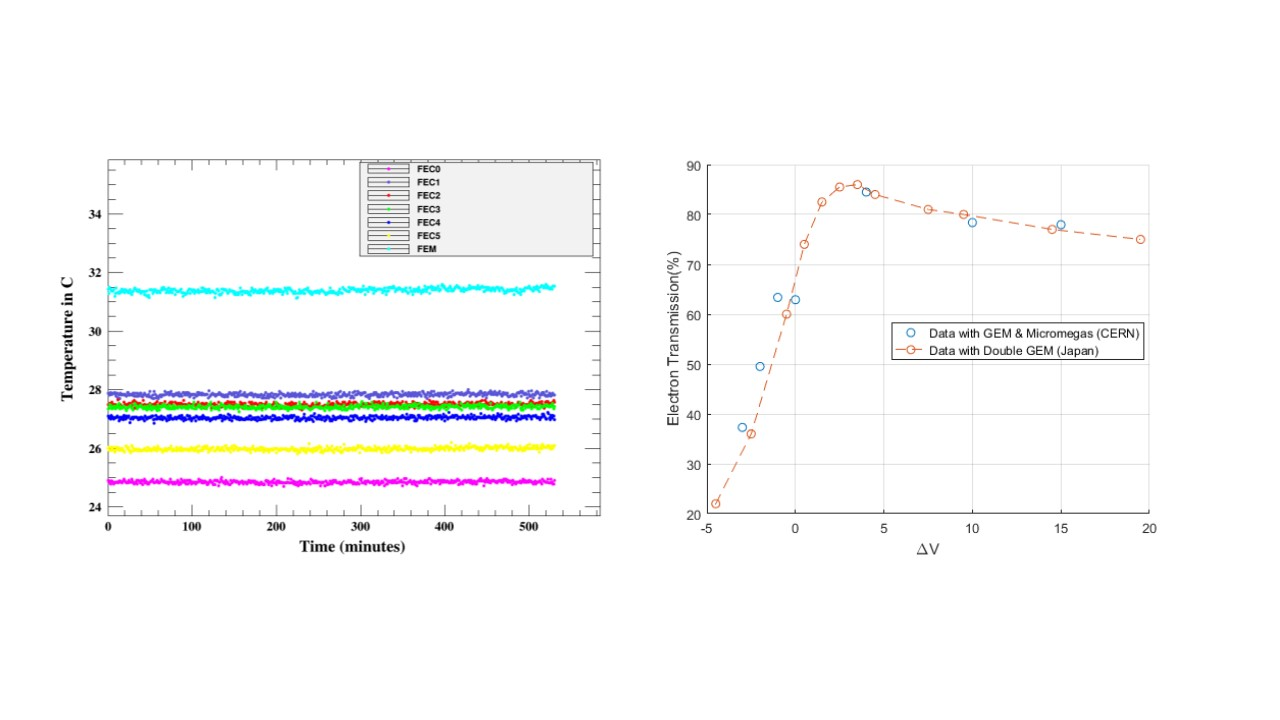
\includegraphics[width=1.0\hsize]{Detector/fig/TPC_operation.jpg}
\caption{TPC operation achievements: temperature stability with double phase $CO_2$ cooling (left) and signal electron transparency with GEM gating (right).} 
\label{fig:det:TPC_operation}
\end{figure}

\vspace{2cm}